\problemname{A Rational Sequence (Take 3)}

A sequence of positive rational numbers is defined as follows:

An infinite full binary tree labeled by positive rational numbers is defined by:
\begin{itemize}
\item The label of the root is $1/1$.
\item The left child of label $p/q$ is $p/(p+q)$.
\item The right child of label $p/q$ is $(p+q)/q$.
\end{itemize}

The top of the tree is shown in the following figure:

% this is the same as https://open.kattis.com/problems/rationalsequence
\begin{figure}[!h]
    \begin{center}
        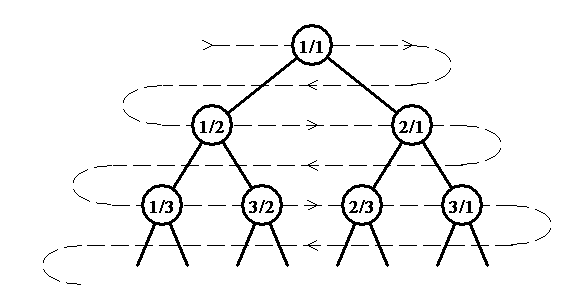
\includegraphics[]{f1.png} \\
    \end{center}
\end{figure}

The sequence is defined by doing a level order (breadth first) traversal of
the tree (indicated by the light dashed line). So that:

\[
F(1) = 1/1, F(2) = 1/2, F(3) = 2/1, F(4) = 1/3, F(5) = 3/2, F(6) = 2/3, \ldots
\]

Write a program to compute the $n^{\text{th}}$ element of the sequence, $F(n)$. Does this problem sound
familiar? Well it should! We had variations of this problem at the $2014$ and $2015$ 
Greater NY ACM ICPC Regionals.

\section*{Input}

The first line of input contains a single integer $P$, ($1 \le P \le 1\,000$), which is the number of data sets
that follow. Each data set should be processed identically and independently.
Each data set consists of a single line of input. It contains the data set number, $K$, and the index, $N$,
of the sequence element to compute ($1 \le N \le 2\,147\,483\,647$).

\section*{Output}

For each data set there is a single line of output. It contains the data set number, $K$, followed by a
single space which is then followed by the numerator of the fraction, followed immediately by a
forward slash (`\texttt{/}') followed immediately by the denominator of the fraction. Inputs will be chosen so
neither the numerator nor the denominator will overflow an $32$-bit \textbf{unsigned} integer.

